
\section{Evaluation of register updates}
\label{sec:stt-derivable}
In this section, we deal with the second computation phase in a first-order register transducer, namely evaluating register updates. We show in Lemma~\ref{lem:derive-register-updates} that the second phase is derivable. As  discussed in the end of Section~\ref{sec:stt}, this completes the proof of our main theorem. 



Our proof uses the language of $\lambda$-calculus.  In Section~\ref{sec:one-register},  we discuss derivability of  evaluation for $\lambda$-terms. In Section~\ref{sec:updates-endgame}, we reduce evaluation of register updates to  unfolding the matrix power  and evaluation of $\lambda$-terms.  

\section{Evaluation of simply typed linear terms}
\label{sec:one-register}

In this section, we consider an important example of derivable term transformations, namely evaluating (i.e.~computing $\beta$-normal forms of)  simply typed  $\lambda$-terms that are linear in the sense that each bound variable is used exactly once in its scope. Apart from its independent interest, evaluation of $\lambda$-terms will  be used in the proof our main theorem. 



\newcommand{\otype}{o}
We assume that the reader is familiar with the basic notions of the simply typed $\lambda$-calculus; more detailed definitions can be found in~\cite{sorensen_lectures_2006}. Define  \emph{simple types} to be expressions  generated from an atomic type $\otype$ using a binary arrow constructor, as in the following examples:
    \begin{align*}
        \otype \qquad \otype \to \otype \qquad (\otype \to \otype) \to (\otype \to \otype) \qquad \cdots 
    \end{align*}
Let $X$ be a set of variables, each one with an associated simple type.  A $\lambda$-term over these variables can be seen as a tree over the ranked alphabet
\begin{align*}
      \overbrace{\set{x : x \in X}}^{\text{arity 0}} \cup \overbrace{\set{\lambda x : x \in X}}^{\text{arity 1}} \cup  \overbrace{\set @}^{\text{arity 2}}
\end{align*}
where @ is the application symbol that is used to apply one term to another.
We say that a $\lambda$-term is \emph{well-typed} if one can associate  to it  a simple type according to the usual typing rules of simply typed $\lambda$-calculus\footnote{
    Here we assume that the variables are typed, but the types for the remaining $\lambda$-terms need to be inferred. We could adopt a different approach, more thoroughly in the style of Church, where all term constructors (application and $\lambda$-abstraction) come decorated with the type of the resulting term. We do not do this to make  notation lighter, and also because one show -- see the appendix -- that first-order logic is enough to reconstruct the type of a term once the types of the variables are known. 
}, see~\cite[Definition 3.2.1]{sorensen_lectures_2006}. Because the variables are typed, a  $\lambda$-term can have either a unique type, or it is not well-typed.  Here is an example of a well-typed $\lambda$-term: 
\mypic{45}
We use the standard notion of $\beta$-reduction for $\lambda$-terms, see~\cite[Definition 1.2.1]{sorensen_lectures_2006}. 
Because of normalisation and confluence for the simply typed $\lambda$-calculus, every well-typed $\lambda$-term has a unique normal form, i.e~a $\lambda$-term to which it $\beta$-reduces (in zero or more steps), and which cannot be further $\beta$-reduced.


\begin{example}\label{ex:exponential}
    Because of iterated duplication, the normal form of a $\lambda$-term can be exponential. Assume that we have two variables $\typevar x  \otype$ and $\typevar y {\otype \to \otype \to \otype}$ and consider the $\lambda$-terms defined by:
    \begin{align*}
        M_0 \eqdef \typevar x \otype \qquad M_{n+1} = (\lambda \typevar x  \otype . \typevar y {\otype \to \otype \to \otype}  \typevar x  \otype \typevar x  \otype)M_n.
    \end{align*}
    The $\lambda$-term $M_n$ is well-typed and of type $\otype$. It has size linear in $n$, but its normal form has size exponential in $n$. 
    % as shown in the following picture, which uses variables $x : \otype$ and  $z : \otype \to \otype \to \otype$.
    % \mypic{44}
\end{example}
As witnessed by the above example, normal forms can be exponential size (or worse, see~\cite[Section 3.6]{sorensen_lectures_2006}), and therefore they cannot be computed  using derivable functions or first-order transductions, because the latter have linear size outputs. To avoid this problem, we  limit attention to linear $\lambda$-terms: a $\lambda$-term is called \emph{linear} if every bound variable is used exactly once in its scope. Here is an example: 
\mypic{43}
For linear $\lambda$-terms, each step of $\beta$-reduction reduces the number of nodes by exactly 3, and therefore the normal form is linear in the size of (in fact, smaller or equal to) the original term. 

Linearity alone is not enough to normalise terms with first-order transductions. Another obstacle is terms that use types of unbounded complexity, as illustrated in the following example. 

\begin{example}
Consider the following $\lambda$-terms, which have types of unbounded size:     \begin{align*}
        M_0 \eqdef \typevar u {\otype \to \otype}  \qquad M_{n+1} \eqdef \overbrace{\lambda \typevar x {\otype}. \lambda \typevar y {\otype}.   M_n (\typevar z {\otype \to \otype \to \otype}  \typevar x {\otype} \typevar y {\otype}).}^{\text{type} \overbrace{\otype \to \otype \to \cdots \to \otype}^{\text{$n+1$ arrows}}}
    \end{align*}
    Apart from having large types (although still of rank 1, as described in~\cite[Exercise 3.6.7]{sorensen_lectures_2006}), these  $\lambda$-terms are simple: they use four variables (although the bound variables are reused), and are linear, because each bound variable is used exactly once in its scope. 
    To $M_n$, apply  $m$ arguments of type $\otype$:
    \begin{align}\label{eq:complicated-term}
    M_n \overbrace{\typevar v \otype \ \typevar v {\otype} \cdots \typevar v{\otype} }^{\text{$m$ times}}.
    \end{align}
    We claim that the above $\lambda$-term cannot be normalised using a first-order transduction, or even a monadic second-order transduction. In order to normalise, a transduction would need to be able to compare the numbers $n$ and $m$ as follows:  if $m < n$  the normal form contains $\lambda$, if $m=n$  the normal form does not contain $\lambda$, and if $m > n$ then the normal form is undefined because the $\lambda$-term is not well-typed.  Whether or not a $\lambda$-term (seen as a tree over a finite alphabet) contains $\lambda$ is a first-order definable property, and first-order definable properties are preserved under inverse images of first-order transductions. Therefore, if normalisation would be a first-order transduction,
then there would be a first-order formula which would be true for terms of the form~\eqref{eq:complicated-term} with $m>n$ and which would be false for terms of the form~\eqref{eq:complicated-term} with $m=n$. Such a formula cannot exist (even if we allow monadic second-order logic), which can be shown using a pumping argument or Ehrenfeucht-Fra\"iss\'e games. 
\end{example}

The above example explains why we need to bound the size of types that occur in subterms, motivating the following definition:  we say that a $\lambda$-term uses only types from a finite set of simple types $\typeset$ if all  subterms have types in $\typeset$.  Once we assume that $\lambda$-terms are linear, use a fixed finite set of bound variables, and use only types from a fixed finite set of simple types, then normalisation can be done by a derivable function, and therefore also by a first-order tree-to-tree transduction: 

\begin{theorem}\label{thm:normalise} Let $X$ be a finite set of simply typed variables, and let $\typeset$ be a finite set of simple types.
    The following tree-to-tree function is derivable (i.e.~it is the tree restriction of a derivable function on terms):
    \begin{align*}
        M \in \text{$\lambda$-terms over variables $X$} \qquad \mapsto \qquad \begin{cases}
            \text{normal form of $M$} & \text{if $M$ is linear, well-typed,}\\
            & \text{and uses only types from $\typeset$;}\\
            M & \text{otherwise}.
        \end{cases}
    \end{align*}
\end{theorem}

% Actually, we prove a stronger result, namely that the above function is derivable. In the end, of course, we will prove that all first-order tree-to-tree transductions are derivable, but our proof of this fact will use the derivability of normalisation as stated in Theorem~\ref{thm:normalise}.



% Recall that elements of $\tmonad \rSigma$ are defined to be trees over $\rSigma + \varnames$, where 
% \begin{align*}
%     \varnames = \set{x_1,x_2,\ldots}
% \end{align*}
% is a fixed set of  variable names that are used for ports. In this section, we view $\varnames$ as a simply typed set, where all variables $x_1,x_2,\ldots$ have the same simple type $\otype$.  Under this convention, we can view
% \begin{align*}
%     \tmonad (\overbrace{\set{x : x \in X}}^{\text{arity 0}} \cup \overbrace{\set{\lambda x : x \in X}}^{\text{arity 1}} \cup  \overbrace{\set @}^{\text{arity 2}})
% \end{align*}
% as a set of $\lambda$-terms. This is exactly the set of those $\lambda$-terms over variables $X + \varnames$ where: (a) variables from $\varnames$ are never bound; and (b) there is some $n$ such that each of the variables $x_1,\ldots,x_n \in \varnames$  appears as a free variable exactly once  and the remaining variables in $\varnames$ do not appear at all. If $S$ is a finite set of simple types, then define  $\linterm S X$ to be those terms in .. which are linear and $S$-typed. 

% Computing the normal form is beyond the scope of first-order transductions, the principal reason being that first-order transductions have linear size outputs, while normalisation can incur a blowup that is exponential or larger,
%  In Section~\ref{sec:lambda}, we will show that normalisation can be computed by a first-order transduction, assuming that: (a) the input terms are linear, which means that each bound variable is used exactly once in its scope; (b) we place an upper bound on the complexity of types used in subterms. 

% as discussed in Example~\ref{ex:labmda-terms}.  We show that the tree-to-tree function which inputs a  term and outputs its normal form can be derived, assuming that bound variables are used exactly one and there is a bound on the number of distinct terms types that can appear in the term. 

% Let $X$ be a typed set, i.e.~a set of variables with associated simple types. As in  Example~\ref{ex:labmda-terms},  we view $\lambda$-terms with variables of $X$ as trees over an ranked alphabet $\lamrank X$. 

% \begin{lemma}
%     For every typed set $X$ and every finite set $S$ of simple types, the tree language 
%     \begin{align*}
%         \set{ M \in \trees \lamrank X : \text{$M$ is well-typed and all subterms have type in $S$}}
%     \end{align*}
%     is first-order definable 
% \end{lemma}



% We say that a function $\ranked f : \linterm S X \rto \linterm S Y$ is \emph{derivable} if it can be extended to a derivable function $\ranked g : \tmonad \lamrank X \rto \tmonad \lamrank X$. The main result of this section is that normalisation is derivable, for every fixed finite $X$ and $S$. 
% \begin{proposition}\label{prop:one-register} 
%     For every typed set $X$ and every finite set $S$ of simple types, the function 
%     \begin{align*}
%         M \in  \linterm S X \qquad \mapsto \qquad \text{normal form of $M$} \in  \linterm S X
%     \end{align*}
%     is derivable.
% \end{proposition}
%


% \paragraph*{Normalisation of non-pure terms.} Let $\rGamma$ be a finite ranked set. Trees over the alphabet $\rGamma+X^\lambda$ are called \emph{$\lambda$-terms over $\rGamma$} or simply \emph{non-pure} $\lambda$-terms.
% Th notions discussed earlier (free and bound variables, $\beta$-reduction and normalization) are the same for non-pure $\lambda$-terms. We suppose that all the element of $\rGamma$ are typed as follows:  the root together with the ports are all of type $\otype$, as illustrated below.
% \begin{center}
% 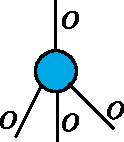
\includegraphics[scale=.4]{pictures/type-gamma}
% \end{center}
% Of course, well-typedeness extends in a natural way. 

% We claim that under the same restrictions, Theorem~\ref{thm:normalise} holds for $\lambda$-terms over $\rGamma$. This follows from this (classical) encoding of the element of $\rGamma$ as pure $\lambda$-terms. 
% Every element  $a \in \rGamma$ of arity $n$ is represented, using  a variable $x_a$ of type 
% \begin{align}\label{eq:low-order-type}
% \overbrace{\otype \to \otype \to \cdots \to \otype}^{\text{$n$ times}} \to \otype
% \end{align}
% as a spine of application nodes of length $n$, ending with the variable $x_a$, as shown below.
% \begin{center}
% 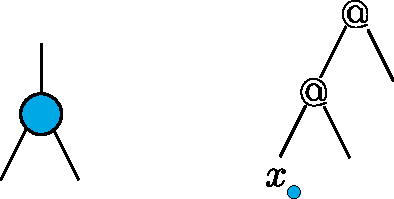
\includegraphics[scale=.4]{pictures/encode-gamma}
% \end{center}
% If a non-pure term satisfies the condition of Theorem~\ref{thm:normalise}, then so does its pure encoding. Indeed, the variables corresponding to $\rGamma$  -- which are not bound -- are the only ones used multiple times.  Furthermore, all sub-terms in the encoding have type of the form~\eqref{eq:low-order-type}, with $n$ being at most the maximal arity of letters in $\rGamma$. Summing up, the encoding of a non-pure $\lambda$-term is linear and can be typed using a bounded set of types, and therefore it falls under the scope of Theorem~\ref{thm:normalise}. 
  
\subsection{Evaluation of register updates}
\label{sec:updates-endgame}
Equipped with Theorem~\ref{thm:normalise}, we  prove derivability of  evaluation of  register updates. 
Fix a first-order register transducer.
% Fix a set of registers names $\regnames$, an output alphabet $\rGamma$, and a finite set $\rDelta$ of monotone register updates.  
From now on, when speaking about register updates or register valuations, we mean those of the fixed transducer. 
Our goal is to prove the following lemma, which completes the proof of our main theorem.
\begin{lemma}\label{lem:derive-register-updates}
    Consider
    the   tree-to-tree function, which inputs a tree of  register updates, evaluates it, and outputs the  contents of the designated output register. This function is derivable. 
    % \begin{eqnarray*}
    % \trees{\ranked{\text{(register updates)}}} &\to & \trees \rGamma \\
    % t & \mapsto & \text{contents of register 1 after evaluating $t$}\\
    % && \text{after evaluating $t$}
    % \end{eqnarray*}    
\end{lemma}
% Theorem~\ref{thm:main}.  
% To prove the lemma, we will model   register updates by evaluation of $\lambda$-terms as in Theorem~\ref{thm:normalise}. %This reduction will involve the matrix power. 

\paragraph*{Output letters in $\lambda$-terms.} We will   use $\lambda$-terms to represent register updates, which involve letters of the output alphabet $\rGamma$. Therefore, for the  rest of Section~\ref{sec:updates-endgame}, we use an extended definition of $\lambda$-terms, which allows  constructing $\lambda$-terms of the form 
\begin{align}\label{eq:non-pure}
a(M_1,\ldots,M_n) \qquad \text{for every $a \in \rGamma$ of arity $n$.}
\end{align}
The typing rules are extended as follows: if the arguments $M_1,\ldots,M_n$ all have type $\otype$ (no other type is allowed for arguments of $a$),  then~\eqref{eq:non-pure} has type $\otype$. These $\lambda$-terms can  be represented as trees, as in the following picture:
\mypic{118}
% We write $\ranked{\rGamma_\lambda}$ for the ranked alphabet used in the tree representation; this is the ranked alphabet from~\eqref{eq:alphabet-for-lambda-terms} plus the output alphabet $\rGamma$. 
Theorem~\ref{thm:normalise} works without change for the extended definition of  $\lambda$-terms used in this section. Note that there is no $\beta$-reduction rule for $\lambda$-terms of the form~\eqref{eq:non-pure}.


\paragraph*{$\lambda$-representations of register updates.}
%  Let $k$ be the number of registers. 
% Register valuations and register updates can be thought of as lists of terms, ordered using the linear order on registers. 
To prove Lemma~\ref{lem:derive-register-updates}, we represent  register updates using a matrix power of $\lambda$-terms. The idea is that the matrix power handles the parallel evaluation of registers.

Let $X$ be a set of variables $\set{x_1\dots,x_m}$, all of them having type $\otype$,  where $m$ is the maximal arity among registers. Define  $\ranked{\Gamma_\lambda}$ to be the output alphabet $\rGamma$ plus the ranked alphabet defined in~\eqref{eq:non-pure} for tree representations of  $\lambda$-terms. 

Recall that a register update -- of arity say $n$ -- consists of a family of terms  over alphabet $\ranked{\Gamma + n\regnames}$, one for each register $r \in \regnames$. We begin by explaining the $\lambda$-representation for terms in the family, which is a function 
 of type
\begin{align}\label{eq:placeholders}
\xymatrix@C=2cm{
    \ranked{\tmonad(\rGamma+n R)} \ar[r]^-{\text{$\lambda$-representation}} &
    \ranked{\tmonad {\Gamma_\lambda}}
}.
\end{align}
This function  is not arity preserving, which is why it is not written in red. Define a  \emph{placeholder} to be an element of $\ranked{n \regnames}$; we write placeholders as $r_i$ with $r \in \regnames$ and  $i \in \set{1,\ldots,n}$.
The function~\eqref{eq:placeholders}  is  explained in the following picture:
\mypic{103}
Note how the  
 arities need not be preserved: the arity of the output is the number of placeholders in the input, which need not be the same as the number of ports in the input. The correspondence of ports in the output term with placeholders in the input term is defined with respect to some arbitrary order on the set $\ranked{n \regnames}$ of placeholders, say lexicographic with respect to the order on registers and  $\set{1,\ldots,n}$.

% We will represent it as a term over  define its $\lambda$-representation to be  of arity $l$, then $\lambda(t)$ is obtained by:
% \begin{enumerate}
% \item[(a)] Replacing the  $i$-th port  of $t$ with the variable $x_i$.
% \item[(b)] Binding all the  variables $x_1,\ldots,x_l$  at the beginning of the term, in this order.
% \item[(c)] Applying the following rewriting rule, where $r_i \in \ranked{nR}$
% \begin{align*}
% r_i(t_1,\dots,t_p) \mapsto @(@(\dots @(\portletter, t_1)\dots,t_{p-1}),t_p)
% \end{align*}
% which replaces every $p$-ary letter $r_i$ by a spine of $@$ of lenght $p$. In particular,when  $r_i$ is nullary, it is replaced by a port.
% This rewriting rules creates, for every name $r_i$, a new port. We call it the \emph{port of $r_i$}.
% \end{enumerate}
% This construction is is illustrated by the following picture.
% \begin{center}
% 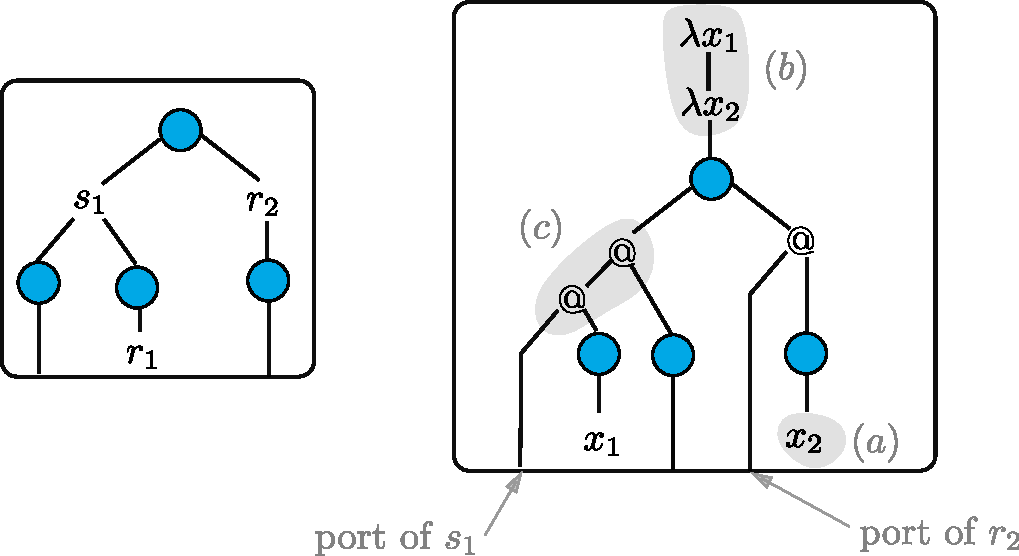
\includegraphics[scale=.33]{pictures/lambda}
% \end{center}

Having defined the $\lambda$-representation of terms with placeholders, we lift it a $\lambda$-representation of  register updates
\begin{align}\label{eq:lambda-representation-regup}
\ranked{
    \xymatrix@C=2cm{
 \text{register updates}    \ar[r]^-{\text{$\lambda$-representation}} &
 \mati k {(\tmonad\Gamma_\lambda)}
}
},
\end{align}
where $k$ is the number of registers. This function is arity preserving. 
For a register update $(t_1,\ldots,t_k)$, where $t_i$ is the term with placeholders used in the $i$-th register,  its $\lambda$-representation is defined to be 
\begin{align*}
(\text{$\lambda$-representation of $t_1$},\ldots,\text{$\lambda$-representation of $t_k$})/f ,
\end{align*}
 where the grouping function $f$ connects a placeholder $r_i$ to the $r$-th sub-port of port $i$. 
Here is a picture
\mypic{119}

% The following example illustrates $\lambda$-representations in the case where we have two registers. To avoid the ambiguities, registers $1$ and $2$ are named $r$ and $s$ respectively in the figure.
% \begin{center}
% 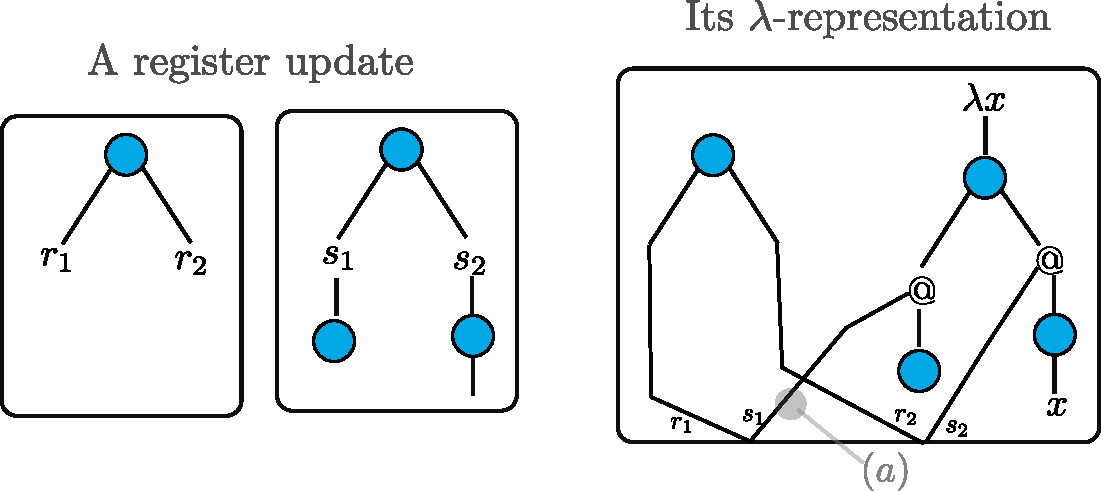
\includegraphics[scale=.33]{pictures/lambda-rep}

% \noindent {\small (a): port of $s_1$ contributes to the second position of the first port in the matrix power.}
% \end{center}
The following  three properties of the $\lambda$-representation for register updates will be used later in the proof:
\begin{enumerate}
\item[(P1)]  If we restrict the domain to a finite set of register updates, e.g.~those used in the transducer, then it is a prime function, by virtue of having finite domain.
\item[(P2)] A register update is monotone  (as in Definition~\ref{def:stt})  if and only if its $\lambda$-representation is monotone (as defined in    Section~\ref{sec:unfolding} for the matrix power).
\item[(P3)] Every bound variable in the $\lambda$-representation is used exactly once, and the types that appear are of the form 
\begin{align*}
\overbrace{\otype \to \otype \to \cdots \to \otype \to \otype}^{\text{at most (maximal arity in $\rGamma$) times}} \to \otype,
\end{align*}
hence Theorem~\ref{thm:normalise} can be applied. 
\end{enumerate}

 
%To get the feeling of this function, we will first present it in the case where the automaton has only one unary regiTheorem~\ref{thm:normalise}.ster. The general case will be presented  in a second step.
%
%\paragraph*{The case of one register (k=1).} There is mismatch between the arity of register updates and the arity of the terms they contain (which is always 1). This is illustrated by the left figure below: the register update is of arity 2, but its content is of arity 1. A consequence of this mismatch is that a term of register updates cannot be seen as a term of terms, and the prime function of flattening and block etc cannot be applied; in other words, the inner structure of register updates is not accessible.
%Let us fix a variable $x$ of type $o$. The $\lambda$-representation, described in the figure below, is intended to bridge this gap, while preserving the behavior of register updates. 
%\begin{center}
%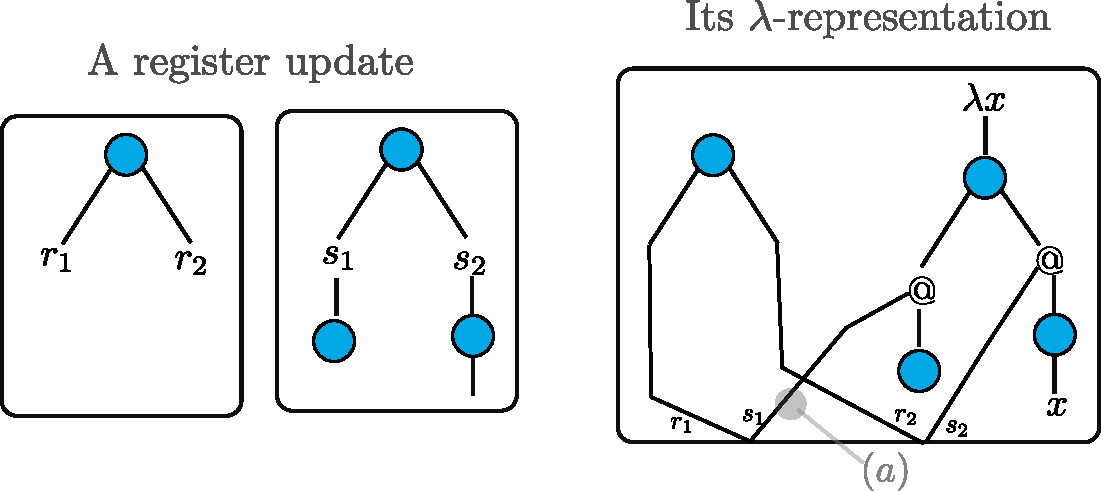
\includegraphics[scale=.36]{pictures/lambda-rep}
%\end{center}
%In words, the $\lambda$-representation transforms the (unique) port of the inner term into $x$ and replaces every letter $r_i$ is by a redex, the pending port of this redex becomes \begin{figure}[]
    
%
%The $\lambda$-representation does not only match the arities between the register update and their content, it also  respects their behavior, as illustrated by the following diagram.
%\begin{center}
%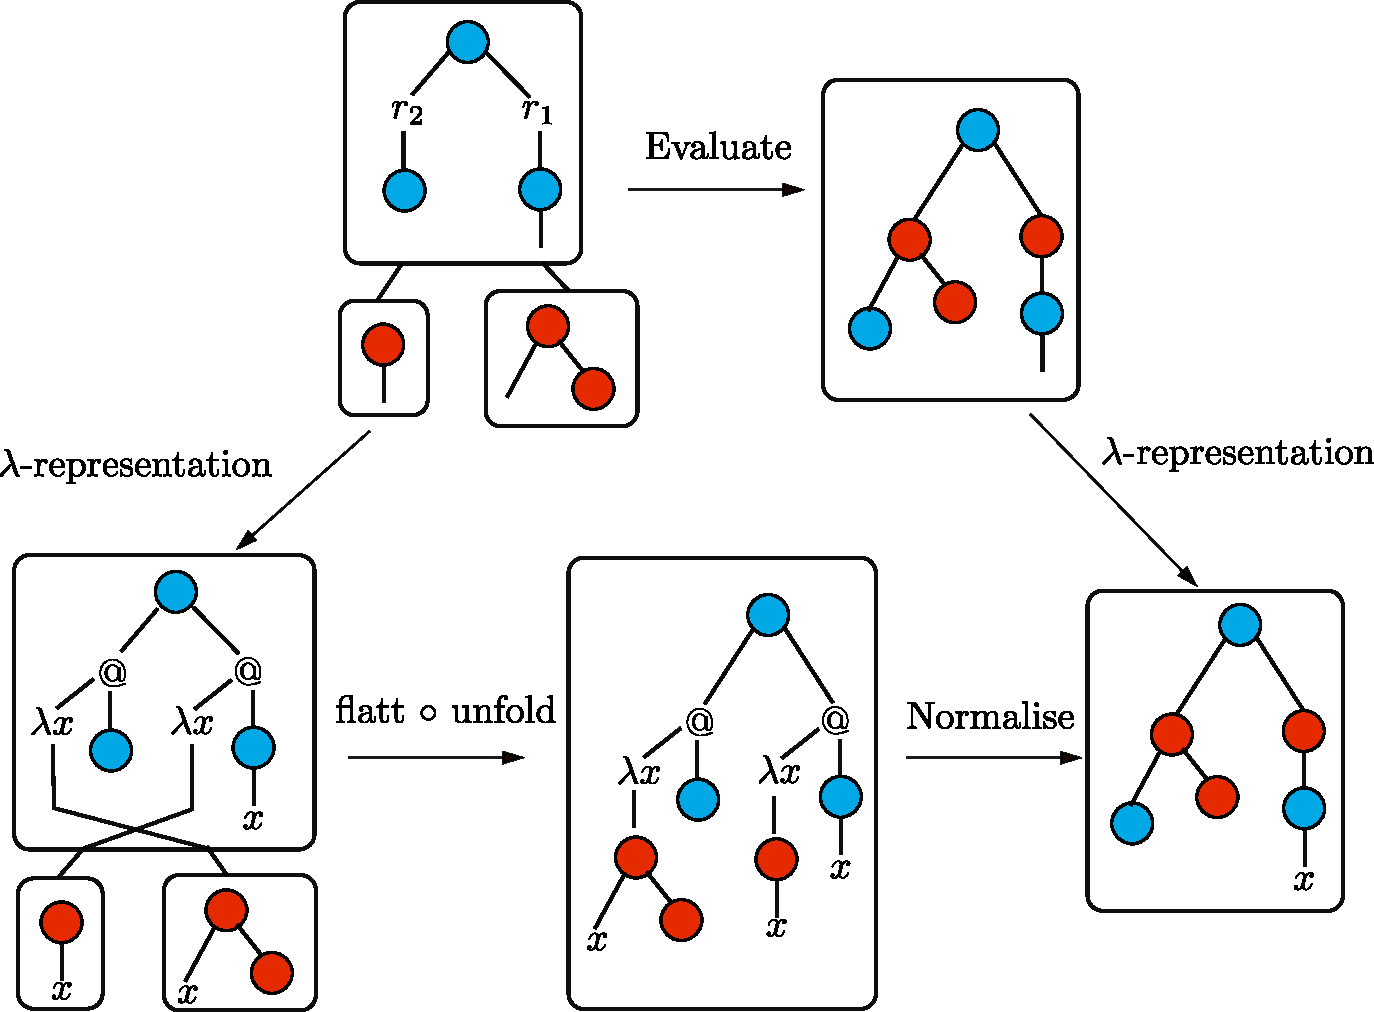
\includegraphics[scale=.36]{pictures/lambda-rep-diagram}
%\end{center}
%In words, the evaluation of a term of register updates can be simulated, through  $\lambda$-representation, by unfolding and normalization functions, which are derivable. 
%
%\paragraph*{The general case.} Let us describe the $\lambda$-representation in the general case. As in the case $k=1$, the inner portes become the variable $x$, every register name becomes a redex. The issue here is how to combine the ports.
%
%\begin{center}
%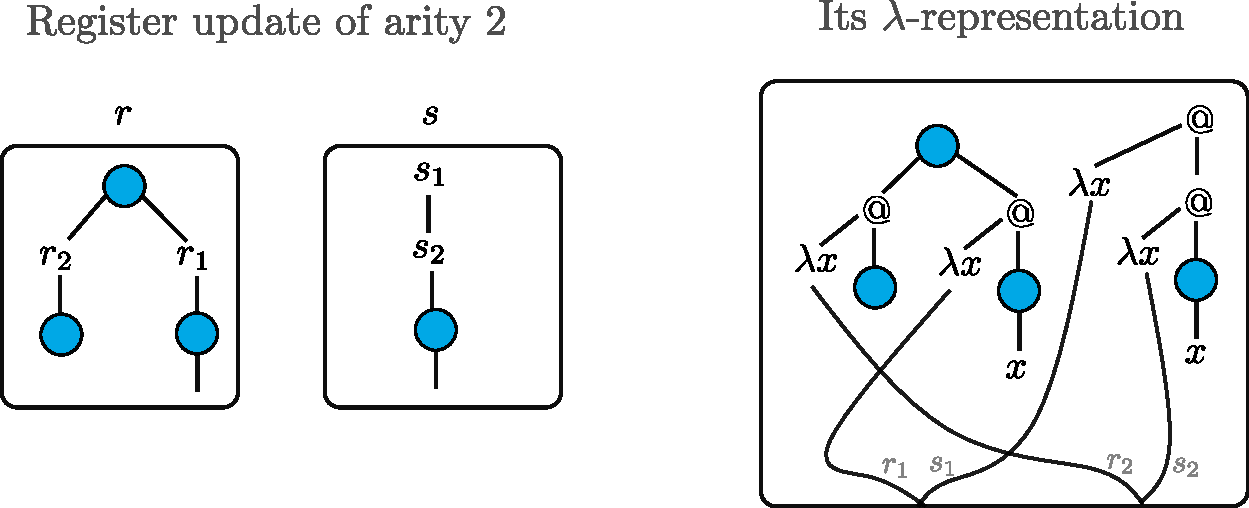
\includegraphics[scale=.36]{pictures/lambda-rep-general}
%\end{center}
% To describe the register updates in a transducer, we will use notions from $\lambda$-calculus.  
% We will also give more precise description of the $\lambda$-calculus in Section~\ref{sec:one-register}; for the moment it is enough to assume that $\lambda$-terms are like trees, except that they allow variables $x,y,z,\ldots$; binding the variables using $\lambda x, \lambda y, \lambda z, \ldots$ and applying one term to another. The evaluation of $\lambda$-terms is performed by $\beta$-reduction
% \begin{align*}
% (\lambda x. M) N \qquad \to_\beta \qquad M[x:=N],
% \end{align*}
% which substitutes a variable by an argument. The $\lambda$-terms that we use are going to be simply typed, which will imply that $\beta$-reduction eventually terminates, arriving at a normal form (called the value of the $\lambda$-term), and this normal form will not depend on the order in which $\beta$-reduction was performed. 
% Define a \emph{$\lambda$-term} to be an expression built using the following grammar
% \begin{align*}
%  \underbrace{x,y,z,\ldots}_{\text{variables}} \quad \underbrace{MN}_{\text{application}} \quad \underbrace{\lambda x.M}_{\text{$\lambda$-abstraction}}.
% \end{align*}
% We use simply typed $\lambda$-calculus. This means that every variable is associated to a type, and we only consider terms which are well-typed. The types that we use are simple types: these 
% Sometimes, we extend the syntax, by allowing a symbols from the output alphabet  $\rGamma$:  terms of the form $a(M_1,\ldots,M_n)$, where $a \in \rGamma$ is a symbol of arity $n$. 

%The red circles in the above picture, which represent nodes of the input term, can be seen  as syntactic sugar: a node with a label  $a \in \rGamma$ of arity $n$ is represented  as a variable of type 
%\begin{align}\label{eq:low-order-type}
%\overbrace{\otype \to \otype \to \cdots \to \otype}^{\text{$n$ times}} \to \otype
%\end{align}
%applied to $n$ arguments. The variables corresponding to $\rGamma$  -- which are not bound -- are the only ones used multiple times; every other variable is used at most once in its scope.   Furthermore, all sub-terms in the $\lambda$-representation have type of the form~\eqref{eq:low-order-type}, with $n$ being at most the maximal arity of letters in $\rGamma$. Summing up, the $\lambda$-representation is affine and can be typed using a bounded set of types, and therefore it falls under the scope of Theorem~\ref{thm:normalise}.

%As discussed in Section~\ref{sec:one-register}, the $\lambda$-representation of a term in $\rGamma$ can be seen as a tree over a finite ranked alphabet; call this ranked alphabet $\ranked{\Gamma_\lambda}$. When the outputs are viewed as trees, the function
%\begin{align}\label{eq:lambda-representation-term}
%\xymatrix@C=2cm{
%    \tmonad \rSigma 
%    \ar[r]^{\text{$\lambda$-representation}} &
%    \trees {\ranked{\Gamma_\lambda}}
%}
%\end{align}
%is not arity-preserving, since all outputs have arity zero. For tree inputs, $\lambda$-representation is the identity function. 

%\paragraph*{The $\lambda$-representation of register updates.} To represent register updates using $\lambda$-terms, we use  the $k$-th matrix power, where  $k$ is the number of registers. The     $\lambda$-representation of register updates is an  arity preserving function, of type
%\begin{align}\label{eq:lambda-representation-regup}
%\ranked{
%    \xymatrix@C=2cm{
% \text{register updates}    \ar[r]^-{\text{$\lambda$-representation}} &
% \mati k {(\tmonad\Gamma_\lambda)}
%}
%}.
%\end{align}
%This function is illustrated in Figure~\ref{fig:labmda-representation-for-register-updates}. 
% \miktodo{Give a definition, maybe?}
%Although most likely this  function is not derivable in general;  it does become derivable if we restrict the domain to a finite set of register updates, by virtue of having a finite domain.





\label{page:monotone-discussed}


\paragraph*{Putting it all together.} To finish the proof of Lemma~\ref{lem:derive-register-updates}, we   observe  that the semantics of a register automaton are translated -- under the $\lambda$-representation -- to unfolding the matrix power and evaluating a $\lambda$-term.  This observation is formalised by saying that the diagram in Figure~\ref{fig:lambda-representation-diagram} commutes, and it  follows directly from the definitions. Instead of giving a proof, we illustrate it on an example in Figure~\ref{fig:lambda-representation-proof}.



\begin{figure}[]
    \centering
    \begin{align*}
        \xymatrix@C=3cm{
            \trees \ranked{\text{(register updates)}} 
            \ar[dd]_{\substack{\text{evaluate}\\\text{register}\\\text{updates}}}^{\text{(a)}}
            \ar[r]^-{\trees(\text{\ranked{$\lambda$-representation}})}_{\text{(c)}}
            &
            \trees \ranked{(\mati k{(\tmonad \Gamma_\lambda)})}
            \ar[d]^{\substack{\text{unfold}\\\text{matrix}\\\text{power}}}_{\text{(d)}} \\
            & 
            \txt{{\tiny arity 0 elements of }\\
            $
            \mati k {\ranked{(\tmonad \Gamma_\lambda)}}
            $}
            \ar[d]^{\substack{\text{evaluate}\\\text{$\lambda$-terms}}}_{\text{(e)}}\\
             \text{register valuations}
            \ar[r]_-{\ranked{\text{$\lambda$-representation}}}^{\text{(b)}}
            &
            \txt{{\tiny arity 0 elements of }\\
            $
            \mati k {\ranked{(\tmonad \Gamma_\lambda)}}
            $}
        }
    \end{align*} 
    \caption{}
    \label{fig:lambda-representation-diagram}
\end{figure}
\begin{figure}[]   
    \hspace{-0.5cm}
    \includegraphics[page=120,scale=0.34]{pics}
    \caption{Example for Figure~\ref{fig:lambda-representation-diagram}.}
    \label{fig:lambda-representation-proof}
\end{figure}
 
\pagebreak 
We claim that all of the arrows (c), (d) and (e) on the  right-down path  in  Figure~\ref{fig:lambda-representation-diagram}  are derivable:
\begin{itemize}
    \item[(c)] Since we work with a fixed register transducer, there is a finite subset $\rDelta$ of register updates  used, and therefore  operation (a) in the figure is derivable by property (P1).
    \item[(d)] Arrow (d) represents the unfolding of the matrix power. By property (P2), the outputs of arrow (c) are monotone, and so we can use the monotone unfolding operation, which is a  prime function and therefore derivable. 
    % One technicality that needs to be explained about arrow (d): after applying monotone unfolding to the output of arrow (c), we get an  arity zero element of 
    % \begin{align*}
    %     \ranked{
    %         \mati k {(\tmonad \rGamma_\lambda)}} = \reduce  k {\powersmall{(\tmonad \rGamma_\lambda)}{k}}.
    % \end{align*}
    % To convert this output into a tuple of trees, we use the last prime function in Figure~\ref{fig:monad} to remove the fold $\reduce k$.
    \item[(e)] Finally, arrow (e) represents the evaluation of $\lambda$-terms. This arrow is derivable by Theorem~\ref{thm:normalise}. The assumptions of this theorem are met by property (P3).
\end{itemize}
Since the arrows (c), (d), (e) are derivable, and the diagram commutes, it follows that  the composition of the arrows (a) and (b) is derivable. In other words, there is a derivable function which maps a tree of register updates to the $\lambda$-representation of the resulting register valuation (when viewing a register valuation as a special case of a register update of arity zero). Finally, to get the contents of the output register, we get rid of the fold in the matrix power by using the last function from Figure~\ref{fig:monad}, and  project onto the coordinate for the output register. 


% If we project the register valuation to the coordinate of the output register, we get the $\lambda$-representation of the output tree, which is the same thing as the output tree, since $\lambda$-representation does nothing for terms of arity zero. \footnote{@Mikolaj: this is true only when we dont see the nodes of lambda representations as a syntactic sugar. This is why I used this lambda terms over $\rGamma$ thing. }

This completes the proof of Lemma~\ref{lem:derive-register-updates}, and therefore also of the main theorem. 




